\documentclass[class=scrartcl, crop=false]{standalone}

\usepackage[sexy]{evan}
\usepackage{nicematrix}
\NiceMatrixOptions{transparent}
\usepackage{array}
\usepackage{pifont}
\newcommand{\cmark}{\ding{51}}%
\newcommand{\xmark}{\ding{55}}%

\title{Notes 10-09}

\begin{document}

\title{Notes 2019-10-09}
\author{Cole Killian}

\section{Case Study: The Cube}


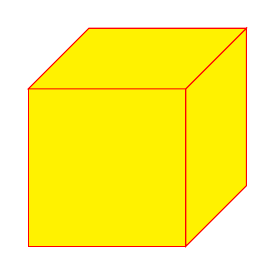
\begin{tikzpicture}
\pgfmathsetmacro{\cubex}{2}
\pgfmathsetmacro{\cubey}{2}
\pgfmathsetmacro{\cubez}{2}
\draw[red,fill=yellow] (0,0,0) -- ++(-\cubex,0,0) -- ++(0,-\cubey,0) -- ++(\cubex,0,0) -- cycle;
\draw[red,fill=yellow] (0,0,0) -- ++(0,0,-\cubez) -- ++(0,-\cubey,0) -- ++(0,0,\cubez) -- cycle;
\draw[red,fill=yellow] (0,0,0) -- ++(-\cubex,0,0) -- ++(0,0,-\cubez) -- ++(\cubex,0,0) -- cycle;
\end{tikzpicture}

8 vertices, 6 faces, 12 edges.

Let $G$ denote the symmetry group of the cube (the same as the isometry or motion group).

This group has 48 elements.

Indeed, there are 8 isometries that map each 

\end{document}

